\section{动量、冲量与过程描述}

牛顿第二定律把某一时刻的受力与加速度联系起来。碰撞、反弹和绳突然绷紧时，力可能在极短时间内剧烈变化，逐时求出力往往既困难也无必要。若研究的是作用前后的速度，就应把运动方程对时间累积，直接建立始末状态之间的关系。这个过程仍以牛顿定律为基础，只是所需的信息从力的瞬时变化转为力的时间积分。

在确定的惯性参考系中，质量为$m$、速度为$\bm v$的质点具有动量$\bm p=m\bm v$。动量是矢量；两次速率相同，并不意味着动量没有变化。例如小球以相同速率撞墙反弹，法向动量反号，其变化量为原法向动量的两倍。计算前应先画出初、末速度，并在同一坐标系中相减，而不能把速率差乘质量当作动量变化。

对质量不变的质点，$\bm F_{\text{合}}=m\dd\bm v/\dd t=\dd\bm p/\dd t$。在$t_1$至$t_2$之间积分，得到
\begin{equation}\bm I_{\text{合}}=\int_{t_1}^{t_2}\bm F_{\text{合}}\dd t=\bm p_2-\bm p_1.\label{eq:em1:impulse}\end{equation}
式中每一项都属于同一个研究对象和同一段时间。某一个力的冲量一般不等于动量变化，只有合力的冲量才直接满足式\eqref{eq:em1:impulse}。若力恒定，可写为$\bm I=\bm F\Delta t$；若力方向固定而大小变化，沿该方向的冲量是$F-t$图线下的有向面积；若方向也变化，则应先分解再积分。

\fig{fig:em1:vector}{同速反弹仍有动量变化；力时图面积给出对应的法向冲量}{\begin{tikzpicture}

\begin{scope}
\draw[world](2,-.9)--(2,2.4);\draw[flow,blue](-.6,1.8)--(1.4,1.8)node[midway,above]{$\bm p_1$};
\draw[flow,blue](1.4,.8)--(-.6,.8)node[midway,above]{$\bm p_2$};
\draw[force,red](1.4,-.1)--(-2.6,-.1)node[midway,below]{$\Delta\bm p$};
\draw[axis](1.6,2.7)--(.3,2.7)node[left]{$+n$};
\end{scope}
\begin{scope}[xshift=5cm]
\draw[axis](0,0)--(3.8,0)node[right]{$t$};\draw[axis](0,0)--(0,2.8)node[above]{$F_n$};
\fill[blue!15](0,0)--(1.5,2.2)--(3,0)--cycle;\draw[world](0,0)--(1.5,2.2)--(3,0);
\node at(1.5,-.7){$I_n=\int F_n\dd t$};\node[below]at(3,0){$\Delta t$};
\end{scope}
\end{tikzpicture}}

图\ref{fig:em1:vector}取离墙的法向$n$为正，故入射$p_{1n}<0$、反弹$p_{2n}>0$，动量变化沿$n$。右图用同一正方向画出接触力的冲量面积；同速反弹时面积对应$2mv$。两速率相等并不使这一矢量差为零。


对一个矢量定理，坐标方向是方程的一部分。例如球以速率$u$竖直向下到达地面，再以速率$w$向上离开；若取向上为正，初、末动量是$-mu,+mw$，故变化量为$m(w+u)$。若改取向下为正，变化量变成$-m(w+u)$，支持力冲量也随之变号，最后得到的力大小相同。正确结果应不依赖人为选定的坐标，但代数过程中必须始终使用同一套方向。

将动量定理写成分量式时，$I_x=m(v_{2x}-v_{1x})$与$I_y=m(v_{2y}-v_{1y})$分别独立成立。只有某方向合外冲量为零，才可说该方向动量不变；另一方向即使存在很大冲量，也不会直接破坏这个结论。固定槽中绳突然绷紧就是典型情形：槽壁可以提供垂直槽的冲量，而沿槽的动量仍可能守恒。先识别能守恒的分量，再选择方程，通常比先写“动量守恒”再补限制更可靠。

\section{平均作用力与冲击近似}

平均力按冲量定义为$\overline{\bm F}=\Delta t^{-1}\int\bm F\dd t$，它给出同样作用时间内产生同样动量变化的恒力。平均力不一定等于力的最大值，也不应无条件用初、末力的算术平均代替。碰撞时间越短，同一动量变化对应的平均冲击力越大，这也是缓冲材料延长停止时间能降低冲击强度的原因。

\fig{fig:em1:pulse-average}{同样面积的矩形与三角形脉冲有相同冲量，但峰值不同}{\begin{tikzpicture}

\foreach \sh in {0,5}{\begin{scope}[xshift=\sh cm]
\draw[axis](0,0)--(3.5,0)node[right]{$t$};\draw[axis](0,0)--(0,2.9)node[above]{$F_n$};\node[below]at(3,0){$\tau$};
\end{scope}}
\fill[blue!12](0,0)rectangle(3,1.2);\draw[world,blue](0,1.2)--(3,1.2)--(3,0);\node[left]at(0,1.2){$I/\tau$};
\fill[red!12](5,0)--(6.5,2.4)--(8,0)--cycle;\draw[world,red](5,0)--(6.5,2.4)--(8,0);
\draw[guide](5,1.2)--(8,1.2);\node[left]at(5,2.4){$2I/\tau$};\node at(6.5,-.7){虚线为平均力$I/\tau$};

\end{tikzpicture}}
图\ref{fig:em1:pulse-average}两种脉冲持续时间均为$\tau$，有向面积均为$I$。矩形峰值等于平均值$I/\tau$，三角形峰值却是它的两倍。因此始末速度与接触时间只能确定平均力；若题目问最大力，还必须给出接触规律或力时曲线。


忽略重力不能只依据“时间很短”这句话。应比较重力冲量$mg\Delta t$与所关注的动量变化，要求$g\Delta t\ll |\Delta v|$。绳突然绷紧时，绳张力的冲量可以有限，而重力和普通摩擦力的冲量可随作用时间趋近于零。但约束的支持力也可能含冲击分量，不能把所有外力都当作普通有限力。槽内质点、固定轴和刚性墙面尤其需要检查外部约束冲量。

画冲量图时，把每个冲量方向标在受作用物体上，再写分量式。若求地面对球的力，向上的支持力与向下的重力必须分别进入方程；若求球对地面的力，最后再使用作用与反作用关系。两者大小相等、方向相反，但属于不同研究对象。

\fig{fig:em1:gravity-impulse}{对球列冲量方程时，支持力与重力分别进入同一个时间区间}{\begin{tikzpicture}

\begin{scope}
\draw[world](-1,0)--(2,0);\draw[world](.5,.45)circle(.45);
\draw[force,blue](.5,-1.3)--(.5,0)node[pos=0,below]{$\bm I_N$};
\draw[force,red](.5,.45)--(.5,.1);\draw[guide,red](.5,.25)--(-.8,-.4);\node[below,red]at(-.8,-.4){$mg\Delta t$};
\draw[flow](-.7,1.8)--(-.7,.6)node[left]{$u$};\draw[flow](1.6,.6)--(1.6,1.8)node[right]{$w$};
\end{scope}
\node[align=left]at(5,1){向上为正\\$I_N-mg\Delta t=m(w+u)$\\$\overline N=mg+\dfrac{m(w+u)}{\Delta t}$};

\end{tikzpicture}}
图\ref{fig:em1:gravity-impulse}的左侧标出冲量方向，右侧保留重力项。只有$g\Delta t\ll u+w$时才可近似略去它。球对地面的冲量与$\bm I_N$相反，须在求出地面对球的冲量后使用作用与反作用关系。


\section{有限接触时间中的力峰值}

冲量确定以后，为什么还不能唯一决定最大接触力？可以建立一个简单而完整的接触模型回答。把固定墙面附近的可恢复形变等效为劲度系数$k$的轻弹簧，小球质量$m$，入射速度$v$，接触开始时形变量$x=0$。以压入墙面的方向为正，在压缩、恢复的接触阶段，运动方程是$m\ddot x=-kx$。
令 $\omega^2=k/m$，试解 $x=\e^{st}$，则 $s^2+\omega^2=0$，两根为 $\pm i\omega$，组合成实数通解 $x=A\cos\omega t+B\sin\omega t$。
链式求导得 $\dot x=-A\omega\sin\omega t+B\omega\cos\omega t$。
初值 $x(0)=0$ 给 $A=0$，$\dot x(0)=v$ 给 $B=v/\omega$，因此
\[x(t)=\frac v\omega\sin\omega t,\qquad\dot x(t)=v\cos\omega t,\qquad\omega=\sqrt{k/m}.\]
再求导得 $\ddot x=(-v\sin\omega t)\omega=-\omega^2x$，与动力学方程相符。到$t=\pi/(2\omega)$时速度为零、形变最大，之后弹性恢复；到$t=\pi/\omega$时形变回到零，球以速度$-v$离开。接触只维持半个振动周期，不能把继续数学振动的负形变部分当成墙面对球的吸引。

\fig{fig:em1:contact}{弹性接触只取非负形变的半周期，支持力按半个正弦变化}{\begin{tikzpicture}

\begin{scope}
\draw[world](3,-.5)--(3,1.4);\draw[spring](1.4,.4)--(3,.4);\draw[world](1,.4)circle(.4);
\draw[flow](.2,1.5)--(1.8,1.5)node[midway,above]{$+x$};\draw[force](1,.4)--(-.2,.4)node[left]{$N$};
\node at(2.2,.9){$k$};\node at(1,-.4){$m$};
\end{scope}
\begin{scope}[xshift=5.3cm]
\draw[axis](0,0)--(4.8,0)node[right]{$t$};\draw[axis](0,0)--(0,2.8)node[above]{$N$};
\draw[world,blue,domain=0:4,samples=80]plot(\x,{2.2*sin(45*\x)});
\draw[guide](0,2.2)--(2,2.2)--(2,0);\node[left]at(0,2.2){$N_{\max}$};
\node[below]at(2,0){$\pi/(2\omega)$};\node[below]at(4,0){$\pi/\omega$};
\end{scope}
\end{tikzpicture}}

图\ref{fig:em1:contact}的墙面对球支持力大小为$N=kx=mv\omega\sin\omega t$。冲量积分中令 $\phi=\omega t$，$\dd t=\dd\phi/\omega$，上下限变为 $0,\pi$，得到
\[
I=mv\omega\int_0^{\pi/\omega}\sin\omega t\,\dd t
=mv\int_0^\pi\sin\phi\,\dd\phi
=mv[-\cos\phi]_0^\pi=2mv,
\]
与反弹的动量变化一致。峰值与平均值分别为
\[N_{\max}=v\sqrt{mk},\qquad\overline N=\frac{2mv}{\pi/\omega}=\frac2\pi N_{\max}.\]
当$k$增大，接触时间按$k^{-1/2}$缩短，峰值按$k^{1/2}$增大，而总冲量不变。由此可见，同样的速度反弹完全可能具有不同接触强度。平均力可由始末动量直接求，峰值必须依赖具体的接触模型。

如果加入阻尼，弹出速率会小于入射速率，接触曲线不再是对称半个正弦；这时仍可用总冲量求平均作用，但不能继续用$\overline N=2N_{\max}/\pi$。若小球原本竖直落到水平面，在接触时重力也存在，应先检查$mg$相对$N$是否足够小，再决定能否用上述无重力的短时模型。忽略条件来自数量级比较，而不是把重力从图上直接删去。

该模型还说明瞬时冲量近似的用途：把墙变得越来越硬时，形变和接触时间趋小，力峰值却趋大，但有限的速度跳变与冲量仍可稳定保留。它提供始末状态的有效描述，并不声称真实物体完全没有形变。若题目改问最大压缩量、接触持续时间或峰值应力，就需要回到有限接触模型。
\section{多阶段运动与内力冲量}

对由若干质点组成的系统，逐个写出动量定理并相加。相互作用的两内力在每一时刻等大反向，因此同一时间区间内的内力冲量相消，得到$\Delta\bm P=\bm I_{\text{外}}$。这里“相消”的是系统总动量方程中的矢量和，并不表示每个物体没有受到内力，也不表示内力不影响系统内部的相对运动。

\fig{fig:em1:internal-impulses}{同一对内冲量在系统总动量方程中相消，各物体的速度仍会改变}{\begin{tikzpicture}

\draw[guide](-.7,-1)rectangle(5,2.1);
\draw[world](0,0)rectangle(1,1);\draw[world](3,0)rectangle(4,1);\node at(.5,.5){$A$};\node at(3.5,.5){$B$};
\draw[force,red](.5,1.4)--(-.5,1.4)node[midway,above]{$\bm J_{B\to A}$};
\draw[force,red](3.5,1.4)--(4.5,1.4)node[midway,above]{$\bm J_{A\to B}$};
\draw[force,blue](0,.5)--(-1.5,.5)node[left]{$\bm I_A^{\rm ext}$};
\draw[force,blue](4,.5)--(5.5,.5)node[right]{$\bm I_B^{\rm ext}$};
\node at(2,-1.5){系统边界包括$A,B$，两内冲量不跨越边界};

\end{tikzpicture}}
图\ref{fig:em1:internal-impulses}对单独物体有$\Delta\bm p_A=\bm I_A^{\rm ext}+\bm J_{B\to A}$、$\Delta\bm p_B=\bm I_B^{\rm ext}+\bm J_{A\to B}$。把它们在同一时间区间相加，红色两项才抵消；蓝色外冲量仍须保留。选择更大系统只是消去了未知内冲量，并没有自动证明总动量守恒。


若一段运动包含加速、断绳、碰撞和滑行，应先在时间轴上标出事件。连续运动段允许速度连续，瞬时冲击段则通常位置不变而速度突变。使用全过程方程可以消去不需要的中间速度；需要某一物体的速度时，再补写该物体或某一阶段的方程。若摩擦力方向始终不变，可以把冲量直接写成$-fT$；若物体发生反向，必须在反向时刻分段，不能把摩擦力从头到尾固定在同一方向。

\fig{fig:em1:stages}{连续段与冲击事件在同一时间轴上衔接，冲击前后位置连续而速度可突变}{\begin{tikzpicture}

\draw[axis](0,0)--(9,0)node[right]{$t$};
\foreach \x/\lab in {0/0,2/t_1,5/t_2,8/t_3}{\draw(\x,-.1)--(\x,.1);\node[below]at(\x,-.15){$\lab$};}
\node at(1,1.1){受力加速};\node at(3.5,1.1){断绳后运动};\node at(6.5,1.1){碰后滑行};
\draw[guide](2,0)--(2,2.2);\node[above]at(2,2.2){断绳：$v^+=v^-$};
\draw[force,red](5,2.1)--(5,.15);\node[above]at(5,2.1){碰撞：$m(v^+-v^-)=J$};
\draw[dim](0,-1)--(8,-1)node[midway,below]{全过程外冲量为各段外冲量之和};

\end{tikzpicture}}
图\ref{fig:em1:stages}中，理想断绳只撤去之后的约束力，本身不产生速度跳变；碰撞则要区分$t_2^-$与$t_2^+$。若全过程的始末动量都已知，可以先累加外冲量消去中间状态，再补需要的局部方程。


系统动量守恒将在下一讲完整展开。本讲中若选取的系统在某方向没有外冲量，就可直接由系统动量定理令该方向总动量变化为零。这一步只给出一个约束；多物体冲击还常需结合不可伸长绳的速度条件。

\section{绳冲量与速度约束}

不可伸长绳在绷紧后要求两端沿绳方向的速度分量相等；这个条件应从几何关系微分得到。令两端位置为$\bm r_A,\bm r_B$，绳绷紧时$(\bm r_A-\bm r_B)^2=L^2$。对时间求导得
\[2(\bm r_A-\bm r_B)\cdot(\bm v_A-\bm v_B)=0.\]
除以$2L$，便得到$(\bm v_A-\bm v_B)\cdot\bm n=0$。它只要求沿绳的相对速度为零，允许两端有不同的垂直绳分量。因此折线绳、斜绳、带槽质点不能未经投影就令两物体速度相等。

\fig{fv:e1:rope}{绳冲量只调整沿绳分量，垂直分量可以保留}{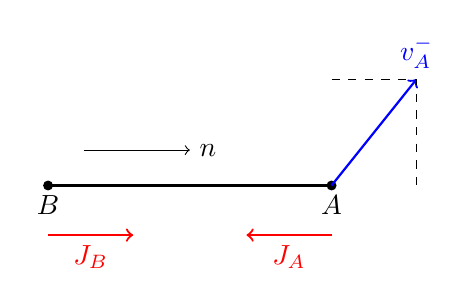
\begin{tikzpicture}[scale=.9]
\draw[thick](0,0)--(4,0);\fill(0,0)circle(2pt)node[below]{$B$};\fill(4,0)circle(2pt)node[below]{$A$};
\draw[->,blue,thick](4,0)--(5.2,1.5)node[above]{$\bm v_A^-$};\draw[dashed](4,1.5)--(5.2,1.5)--(5.2,0);
\draw[->,red,thick](4,-.7)--(2.8,-.7)node[midway,below]{$\bm J_A$};\draw[->,red,thick](0,-.7)--(1.2,-.7)node[midway,below]{$\bm J_B$};
\draw[->](.5,.5)--(2,.5)node[right]{$\bm n$};\end{tikzpicture}}
图\ref{fv:e1:rope}中两冲量等大反向，故总动量不变；各自又都沿绳，故不能改变垂直绳的速度分量。绷紧后的条件只是 $\bm v_A^+\cdot\bm n=\bm v_B^+\cdot\bm n$，并非两个速度矢量完全相同。先用这一投影条件解冲量，再检查冲量确为拉向对方，最后比较初末动能，便能同时区分守恒量、几何约束和非弹性耗散。


理想不可伸长模型只规定几何约束，并不自动保证机械能守恒。松绳绷紧通常相当于沿绳方向的非弹性约束冲击，相对径向动能减少。因此解完速度后可计算动能变化作核验，不能同时强加“总动能不变”而使方程矛盾。

冲击结束后还应检查绳是否需要拉而不是推。设按“绳绷紧”求得的冲量为$J$，约定拉力方向对应$J\ge0$；若解得$J<0$，说明这一约束状态不能由柔绳维持，应改为松弛状态。若只接触而不粘连的物体，法向冲量同样只能把双方推开。速度方程给出候选状态，单侧约束的符号条件决定它是否真实发生。



\subsection{用相对运动能量检验绳收紧}
对图\ref{fv:e1:rope}的两个自由质点，质量分别为$m_A,m_B$。令绷紧前沿绳的分离速度为$u_n=(\bm v_A^- -\bm v_B^-)\cdot\bm n>0$，拉力冲量为$J$。两物体的沿绳速度变化分别为$-J/m_A$与$J/m_B$，故
\[
0=u_n-J\left(\frac1{m_A}+\frac1{m_B}\right),\qquad
J=\mu_r u_n,\quad \mu_r=\frac{m_Am_B}{m_A+m_B}.
\]
质心动量与垂直绳的速度分量均保持不变。记两球原来的沿绳分量为 $v_{An}^-,v_{Bn}^-$，将冲击后的分量 $v_{An}^- -J/m_A$、$v_{Bn}^-+J/m_B$ 分别平方，减去初动能，得
\begin{align*}
K^+-K^-&=-Jv_{An}^-+Jv_{Bn}^-
+\frac{J^2}{2m_A}+\frac{J^2}{2m_B}\\
&=-Ju_n+\frac{J^2}{2\mu_r}.
\end{align*}
代入 $J=\mu_ru_n$，便知消失的只是沿绳相对运动能量：
\[
K^- -K^+=\frac12\mu_r u_n^2\ge0.
\]
这里$\mu_r$是约化质量，不是摩擦系数。若$u_n<0$，两端正相互靠近，候选$J<0$要求绳推物体，故不会发生这种拉紧冲击。若$u_n=0$，瞬时冲量为零，后续是否持续绷紧还须由动力学检验张力。

动量定理本身没有规定能量损失机制。上面的损失来自“绷紧后沿绳相对速度为零”的非弹性模型；若接触可恢复、会反弹，就应换用相应恢复规律。连续接入的链条也可能耗散，外力输入功不必全部成为已运动部分的动能。

\section{连续流与变质量系统}

喷流、雨滴和吸附微尘的飞船，若只盯住装置本身，就会看到质量随时间变化。这时不能把恒质量质点的$\bm F=m\bm a$直接照搬。一个稳妥方法是在极短时间$\dd t$内，选取“装置加上即将流入的那一小团物质”作为封闭系统，写出它在同一惯性系中的初、末动量。

设装置瞬时质量为$M$，速度为$\bm V$；流入质量为$\dd m>0$，其入射速度为$\bm u$。完全并入后，系统末动量为$(M+\dd m)(\bm V+\dd\bm V)$。初动量为$M\bm V+\bm u\dd m$，末动量减初动量为$M\dd\bm V+(\bm V-\bm u)\dd m+\dd m\dd\bm V$。令它等于外冲量，再略去二阶乘积$\dd m\dd\bm V$，得
\begin{equation}M\dd\bm V=\bm F_{\text{外}}\dd t+(\bm u-\bm V)\dd m.\label{eq:em1:inflow}\end{equation}
其中$\dd m/\dd t$必须由相对穿过边界的速度求出。密度$\rho$、横截面积$S$的均匀静止尘区，被以速度$V$飞行的飞船扫过时，单位时间吸附$\rho SV$的质量；每单位质量又需从零加速到$V$，故维持速度所需的附加推力为$\rho SV^2$。

\fig{fig:em1:swept-volume}{静止尘区中的流入量由飞船扫过的体积确定}{\begin{tikzpicture}

\draw[world](0,0)rectangle(2.5,1.5);\node at(1.25,.75){飞船$M$};
\draw[fill=blue!15](2.5,0)rectangle(3.7,1.5);\draw[guide](3.7,-.4)--(3.7,2);
\foreach \x in {2.7,3,3.3,3.6}\foreach \y in {.3,.7,1.1}{\fill(\x,\y)circle(.025);}
\draw[flow](.7,2)--(2.3,2)node[midway,above]{$V$};
\draw[dim](2.5,-.5)--(3.7,-.5)node[midway,below]{$V\dd t$};\node[right]at(3.7,1){截面积$S$};
\node at(1.8,-1.3){$\dd m=\rho S V\dd t$，尘埃对地速度为零};

\end{tikzpicture}}
图\ref{fig:em1:swept-volume}的蓝色薄柱原本静止，体积为$SV\dd t$。完全吸附后，这部分物质具有与飞船相同的速度，所以额外动量增加量是$V\dd m$。若保持$V$恒定，推力必须提供这一项，得到$F=\rho SV^2$，并非把尘埃质量重复计入加速度项。


对固定平面，数密度为$n$、分子质量为$m$、垂直速度为$v$的单向分子束，在$\dd t$内到达面积$S$的分子数为$nvS\dd t$。每个分子镜面反弹后法向动量变化为$-2mv$，平面得到的反向冲量为$2nmv^2S\dd t$。所以压强为$2nmv^2$。若分子被吸收，系数变为$1$；若气体各向运动，就应按速度分布求平均，不能把单向束公式当作平衡气体公式。

\fig{fig:em1:flux}{用同一批物质比较并入前后的动量，质量流率另由穿越边界的相对速度确定}{\begin{tikzpicture}

\begin{scope}
\draw[guide](-.6,-.7)rectangle(3.7,1.5);\draw[world](1.2,0)rectangle(3,.8);\node at(2.1,.4){$M$};
\fill(.1,.4)circle(2pt)node[below]{$\dd m$};\draw[flow](-.7,1.05)--(.8,1.05)node[midway,above]{$\bm u$};
\draw[flow](3.1,.4)--(4.1,.4)node[right]{$\bm V$};\node at(1.6,-1.25){初态：$M\bm V+\bm u\dd m$};
\end{scope}
\begin{scope}[xshift=6cm]
\draw[guide](-.4,-.7)rectangle(3.5,1.5);\draw[world](.4,0)rectangle(2.8,.8);\node at(1.6,.4){$M+\dd m$};
\draw[flow](2.9,.4)--(4,.4)node[right]{$\bm V+\dd\bm V$};
\node at(1.6,-1.25){末态：$(M+\dd m)(\bm V+\dd\bm V)$};
\end{scope}
\end{tikzpicture}}

图\ref{fig:em1:flux}虚线圈住前后同一批物质；左图示意物质从后方追上装置，右图它已完全并入。初末动量统一使用惯性系速度，$\dd m$的大小则由物质实际穿越装置边界的速度决定。两种速度承担不同的计算任务。


对于固定的控制区域，入口与出口可以同时存在；定常时区域内动量不随时间改变，仍有$\bm F_{\text{外}}=\dot m(\bm v_{\text{出}}-\bm v_{\text{入}})$。若控制边界本身移动，穿过边界的质量流率要用流体相对边界的法向速度，而出、入动量必须用同一个惯性系的速度。移动反射板的两个速度用途不同，正需要在图中分别表示。流率乘速度差的量纲为力，也可作为计算后的第一项核验。

\fig{fig:em1:control-volume}{固定控制区中物质进出，区域内动量不变仍可存在非零外力}{\begin{tikzpicture}

\draw[guide](1,-.8)rectangle(5,2.3);\draw[flow,blue](-.5,0)--(2.2,0)node[midway,above]{$\bm v_{\rm in}$};
\draw[world](2,0)..controls(3.1,0)and(3.7,.5)..(4,1.3);\draw[flow,blue](4,1.3)--(4.5,2.5)node[right]{$\bm v_{\rm out}$};
\draw[force,red](3,.4)--(2.2,1.7)node[left]{$\bm F_{\rm on\ fluid}$};
\node at(3,-1.4){定常时$\dot m_{\rm in}=\dot m_{\rm out}=\dot m$};

\end{tikzpicture}}
图\ref{fig:em1:control-volume}中虚线区域内的水不断被替换。虽然其中动量总量保持不变，每秒流出的动量仍不同于流入的动量，导流板必须提供差值$\dot m(\bm v_{\rm out}-\bm v_{\rm in})$。求水对板的力时再反向；若入口、出口压强不同，还必须把压力作用计入外力。


\section{边界动量流与局部受力}

处理连续介质时，一个常见混淆是把“边界内的动量改变”与“穿过边界的动量流”当成同一项。以接收链条的秤盘为例，堆在盘里的链节都静止，盘内总动量近似为零，但链节不断携带向下动量流入。盘必须对进入的链节提供使其停止的冲量，所以仍有额外冲击载荷。若在短时间内改选即将落盘的那段链为封闭系统，就能在普通动量定理中直接看到这一项。

\fig{fig:em1:chain-arrival}{盘内链条已静止，入盘链节仍带来额外的动量流}{\begin{tikzpicture}

\draw[world](-1,0)--(-1,-.4)--(2.5,-.4)--(2.5,0);\draw[world](.1,0)--(.1,2.8);
\foreach \y in {.2,.5,.8,1.1,1.4,1.7,2,2.3,2.6}{\draw[world](.1,\y)ellipse(.1 and .15);}
\draw[world](.1,0)..controls(.6,.4)and(.8,-.3)..(1.2,0)..controls(1.5,.3)and(1.8,-.3)..(2.1,0);
\draw[guide](-.5,.8)--(2,.8);\draw[flow,blue](.8,2.7)--(.8,1.5)node[right]{$v$};
\draw[force,red](1,-1.6)--(1,-.4)node[pos=0,below]{$N$};\draw[force](1.6,.05)--(1.6,-.9)node[right]{$M_pg$};
\node[right]at(2,1.1){边界每秒进入$\lambda v$};

\end{tikzpicture}}
图\ref{fig:em1:chain-arrival}用$M_p$表示已停在盘上的链质量。若进入的链节在线密度$\lambda$不变时以速率$v$竖直下落，并在很短区域内停止，每秒需消去向下动量$\lambda v\cdot v$。因此盘对链的支持力近似为$N=M_pg+\lambda v^2$。第一项支承静止链重，第二项来自入流的制动，两项不能互相替代。这里未计秤盘自重；若链条接触前受到明显张力，应先重新求入流速度。


连续流公式也有有效范围。流入物若会提前互相牵制，或者链条的弯曲部分有不可忽略的张力，就不能继续假设每一链节在撞上前自由下落。短时间近似的重点不是机械地令所有小量为零，而是保留一阶动量流、舍去二阶乘积，并交代物质的入、出状态。

